\documentclass[twocolumn]{article}
\usepackage{amsmath}
\usepackage[utf8]{inputenc}
\usepackage{graphicx}
% \usepackage{subequations}

\def\npup{\ensuremath{U}}
\def\nmaj{\ensuremath{M}}
\def\nprof{\ensuremath{S}}
\def\ngrad{\ensuremath{P}}
\def\ngrant{\ensuremath{G}}
\def\nisi{\ensuremath{P^\text{I}}}
\def\nscielo{\ensuremath{P^\text{S}}}

\def\nal{\ensuremath{N_\text{pub}}}
\def\nal{\ensuremath{N_\text{alumnos}}}
\def\nal{\ensuremath{N_\text{alumnos}}}


\usepackage{geometry}
\geometry{left=16mm,top=16mm,right=20mm,bottom=20mm}

\title{Direct State funding of Chilean universities}
\author{Régis Lachaume}

\begin{document}

\maketitle

\section{Determination}
\subsection{Total funding}
The total funding in year $n$, that we note $F_{n}$, is a slowly increasing series (see Fig.~\ref{fig:total-afd}). In half of the years it approximately follows the consumer price index, but it has received a modest boost in other years.  The average inflation-corrected increase has been $2.3$\% per year in period 2006--2019. This increases matches the increase in undergraduate students ($+2.2\%$ in 2006--2018), real wages ($+2\%$?), and GDP per capita ($+2.xx$\%?). Increase in standard of living and student population are long-term trends that I would expect to hold for at least the next decade, so we can safely assume that University funding by the State will still follow this trend.

For predictions, beyond 2019, I will therefore assume that
\begin{equation}
    F_{n+1} = F_n (1 + q) \label{eq:F}
\end{equation}
where $q = 2$\%.

\subsection{Yearly evaluation}
\label{sec:metrics}

Art. 2 of Decree with Force of Law 4 of 1980, with modifications from Art. 1 of Ministry of Education Decree 116 of 2002, indicates that part of the funding of University $i$ in year $n+1$ is related to metrics measured in year $n$. They involve 
\begin{itemize}
\item $\npup_{i,n}$, the number of undergraduate students (``estudiantes de pregrado'');
\item $\nmaj_{i,n}$, the number of majors (``carreras'');
\item $\nprof_{i,n}$, the number of equivalent full-time scholars (``académicos''), i.e. professors and researchers ;
\item $\ngrad_{i,n}$, the number of equivalent full-time scholars with a post-graduate title such as master of PhD; 
\item $\ngrant_{i,n}$, the number of research grants (``proyectos'');
\item $\nisi_{i,n}$, the number of Web of Science publications (WoS)\footnote{At the time of the Decree 116 it was known as ISI}; 
\item and $\nscielo_{i,n}$, the number of non-WoS publications indexed by the Scientific Electronic Library Online (Scielo) Chile. 
\end{itemize}

The metrics, defined in the aformentioned decrees, are ratios meant to measure an output v. staff efficiency\footnote{While the number of publications is defined by the number of WoS plublications plus one third of Scielo one by Ministry of Education Decree 116 of 2002, the Ministry has consistently used factor 0.33 instead of 1/3 for the calculation.}
\begin{subequations}
\begin{align}
    x_{i,n,1} &= \npup_{i,n} / \nmaj_{i,n},  \label{eq:x1}                          \\
    x_{i,n,2} &= \npup_{i,n} / \nprof_{i,n},                           \\ 
    x_{i,n,3} &= \ngrad_{i,n} / \nprof_{i,n},                          \\
    x_{i,n,4} &= \ngrant_{i,n} / \nprof_{i,n},                         \\
    x_{i,n,5} &= (\nisi_{i,n} + \frac{33}{100} \nscielo_{i,n}) / \nprof_{i,n}
\end{align}
\end{subequations}

According to Art. 3 of Ministry of Education Decree 128 of 1991,  the
evaluation formula renormalises the aforemention ratios in this
way\footnote{Although not specified by the decree, the Ministry has
consistently used the population variance, not the sample variance, for the calculation.} :
\begin{subequations}
\begin{align}
    \mu_{n,k}    &= \frac1n\sum_j x_{j,n,k}\\
    \sigma_{n,k} &= \sqrt{\frac 1n \sum_j \left(x_{j,n,k} - \mu_{n,k}\right)^2 }\\
    y_{i,n,k}    &= \exp \left[ -\frac 95 + \frac14 \frac{x_{i,n,k} - \mu_{n,k} }{\sigma_{n_k}} \right]^3 \label{eq:transform}
\end{align}
\end{subequations}
The transform in Eq.~\ref{eq:transform} ensures that Universities are compared by how much they deviate from
the mean.  Figure~\ref{fig:transform} displays the exponential nature of the rating.

\begin{figure}
\centering
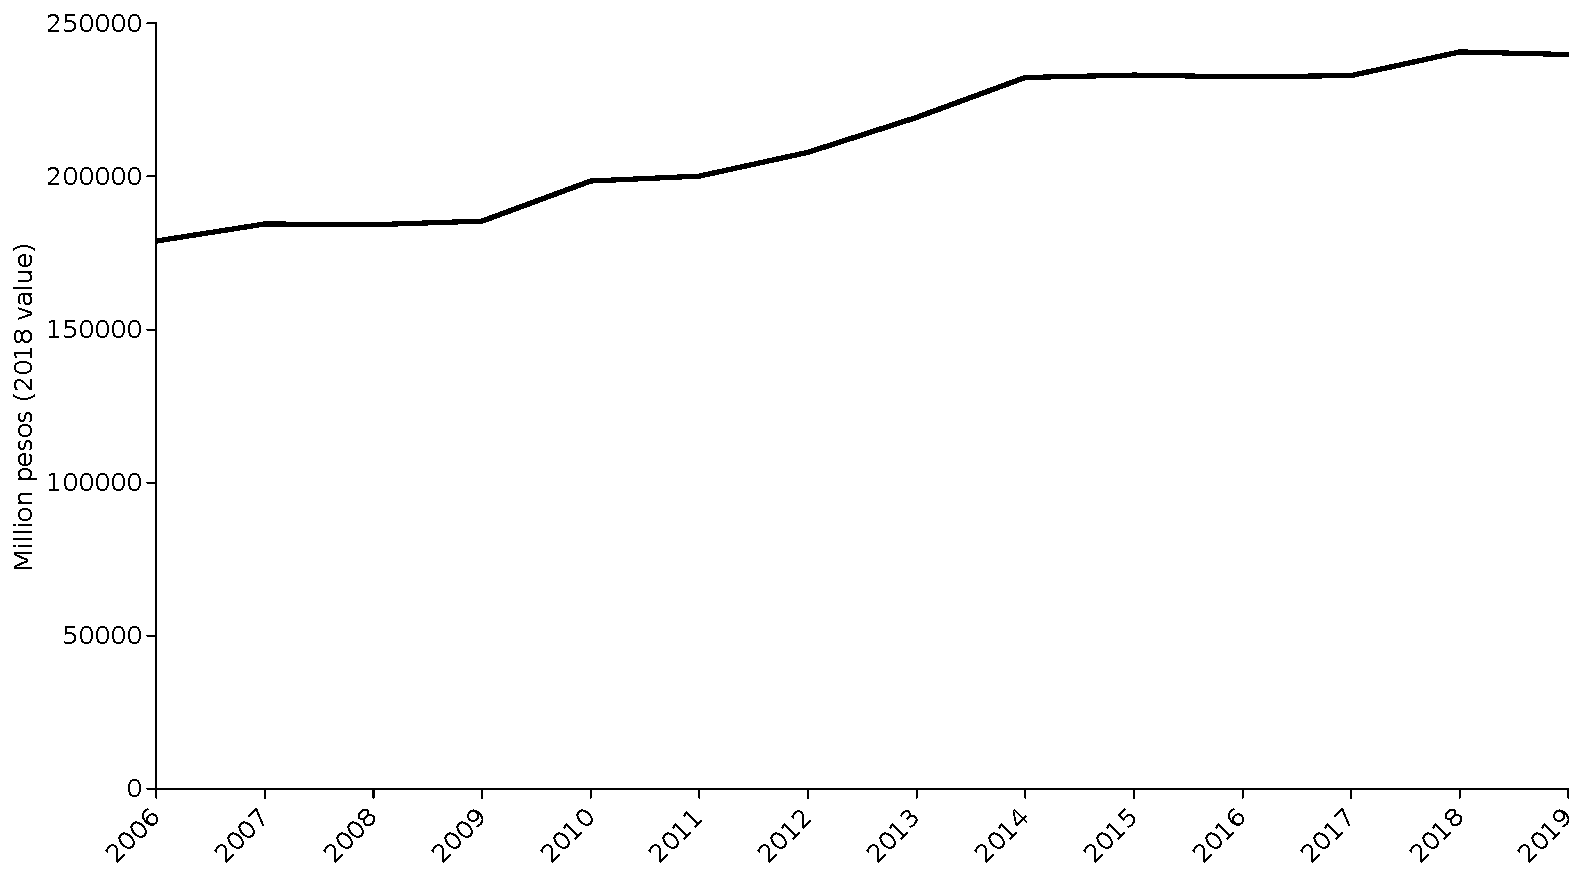
\includegraphics[width=\linewidth]{total-afd-timeseries.pdf}
\caption{Evolution of total direct State funding to Chilean Universities, in 2018
pesos (inflation-corrected).}
\label{fig:total-afd}
\end{figure}

\subsection{Time-evolution for each university}
\begin{table}
\centering
\caption{Coefficients used for university evaluation since 1998.}
\label{tab:coeff}
\begin{tabular}{lll}
\hline\hline
      & ratio                   & value\\
\hline
$c_1$ & students-to-majors      & 0.01\\
$c_2$ & students-to-staff       & 0.14\\
$c_3$ & postgrad staff-to-staff & 0.24\\
$c_4$ & grants-to-staff         & 0.25\\
$c_5$ & papers-to-staff         & 0.35\\
\hline
\end{tabular}
\end{table}

Let $F_{i,n}$ be the funding received by university $i$ at year $n$. Art. 2 of
Decree with Force of Law 4 of 1980 indicates that 5\% of the funding is indexed
on metrics $y_{i,n,k}$ (k in $1\cdots5$) measured for year $n$ (see
Sect.~\ref{sec:metrics}). These metrics are assigned weights $c_k$ which may
vary from year to year, but have been constant since 1998 (see
Table~\ref{tab:coeff}). 95\% of the funding is related to the previous year's
share of the total funding.  So,

\begin{align}
    F_{i,n+1} &= \left( \frac{19}{20} \frac{F_{i,n}}{F_{n}} 
                      + \frac 1{20} \sum_k c_k \frac{y_{i,n,k}}{\sum_j y_{j,n,k}} 
                \right) F_{n+1}.
        \label{eq:afd}
\end{align}


\subsection{Checks}
\begin{figure}
\centering
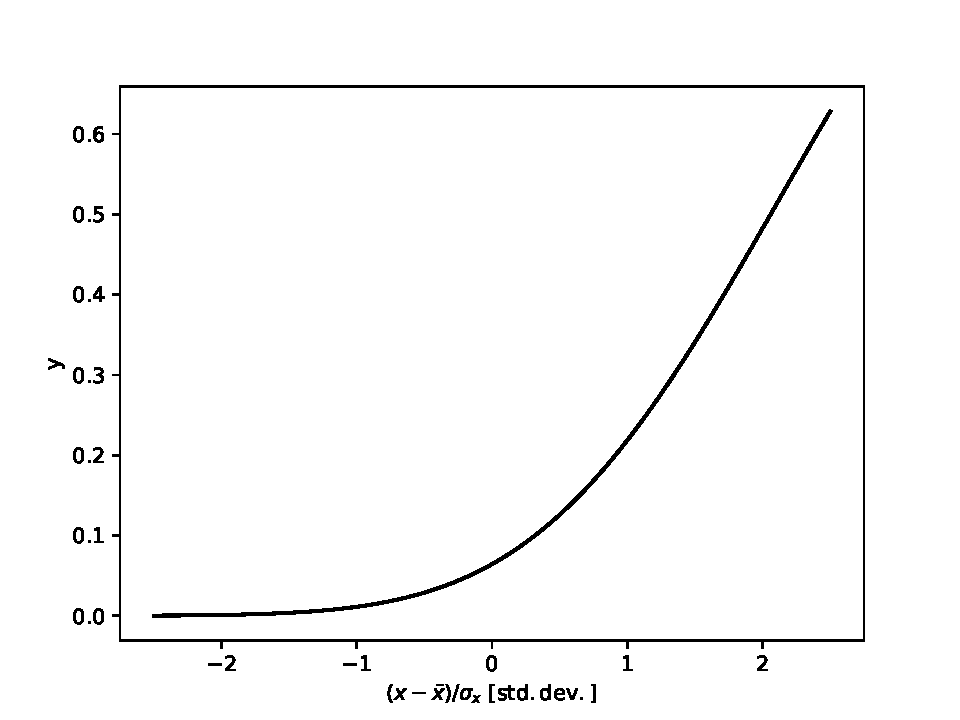
\includegraphics[width=.85\linewidth]{transform.pdf}
\caption{Transformation of the metric $x_{i,n,k}$ into $y_{i,n,k}$, before a weighted sum 
$\sum_k c_{i,n,k} y_{i,n,k}$ is performed to determine the rating of university $i$ in year $n$.}
\label{fig:transform}
\end{figure}

I have checked the calculations using open data from the Eduction Ministry for
years 2006 to 2018. For each year since 2011 and 2007--2009, the percentages I
derived (see Table~\ref{tab:calcdetail} for 2018) match within numerical
rounding errors (8 digits) with those of the Ministry. The subsidies I predict
for each university differ by at most CLP 1,000 (USD 1.50) with the
official ones due to rounding errors, as the accounting unit used in the
official documents is 1,000 Chilean pesos. In 2010, the Ministry used the 2009
calculation with 2008 metrics, instead of 2009 ones. In 2006, there is an
unexplained 0.01\% discrepancy between my determination and the Ministry's. 

The detail of calculations for year 2018 is given in Appendix.~\ref{sec:2018}.
For that year, my calculations match exactly the Ministery's to the peso.

\section{Value of a paper}
\begin{table}
\centering
\caption{University earnings in 2018 Chilean pesos for an additional 
WoS paper in 2017, assuming that the total State funding increases 
2\% per  year in real terms.}
\label{tab:papercost}
\begin{tabular}{lrr}
\hline\hline                             
university                   &  first year &  all years\\              
\hline                                                        
U. de Chile                  &    493\,000 &  15\,903\,000\\  
P. U. Católica de Chile      &    497\,000 &  16\,032\,000\\
U. de Concepción             &    612\,000 &  19\,742\,000\\
U. Católica de Valparaíso    & 1\,658\,000 &  53\,483\,000\\
U. Téc. Fedérico Sta. María  & 1\,328\,000 &  42\,839\,000\\
U. de Santiago               &    407\,000 &  13\,129\,000\\
U. Austral                   &    673\,000 &  21\,710\,000\\
U. Católica del Norte        &    930\,000 &  30\,000\,000\\
U. de Valparaíso             &    456\,000 &  14\,710\,000\\
U. de Antofagasta            & 1\,172\,000 &  37\,806\,000\\
U. de la Serena              &    969\,000 &  31\,258\,000\\
U. de Bio Bio                &    600\,000 &  19\,355\,000\\
U. de la Frontera            & 2\,582\,000 &  83\,290\,000\\
U. de Magallanes             & 1\,107\,000 &  35\,710\,000\\
U. de Talca                  & 1\,674\,000 &  54\,000\,000\\
U. de Atacama                &    395\,000 &  12\,742\,000\\
U. de Tarapacá               & 2\,273\,000 &  73\,323\,000\\
U. Arturo Prat               &    133\,000 &   4\,290\,000\\
U. Metropolitana             &    152\,000 &   4\,903\,000\\
U. de Playa Ancha            &    176\,000 &   5\,613\,000\\
U. Tecnológica Metropolitana &    334\,000 &  10\,744\,000\\
U. de Los Lagos              &    266\,000 &   8\,581\,000\\
U. Católica de Maule         &    317\,000 &  10\,226\,000\\
U. Católica de Temuco        &    290\,000 &   9\,355\,000\\
U. C. de la Sant. Concepción &    213\,000 &   6\,871\,000\\
U. de O'Higgins	             & 8\,565\,000 & 276\,290\,000\\
U. de Aysén                  & 7\,096\,000 & 228\,903\,000\\
\hline
\end{tabular}
\end{table}
If an additional paper is published by a researcher of University $i$ in year $n$, it will reflect in 
the 5\% funding of year $n + 1$. Let us call $\Delta F_{i,n+1}$ the additional earnings 
of the university in that year.  In the subsequent years, it will reflect via the 95\% 
(first term of the right handside of Eq.~\ref{eq:afd}) in this way:
\begin{align}
   \Delta F_{i,n+k} &=  \frac{19}{20} \Delta F_{n+k-1} F_{n+k}  / F_{n+k-1}, \notag\\
\intertext{so, using Eq.~(\ref{eq:F}),}
   \Delta F_{i,n+k} &= \Delta F_{n+k-1}  \frac{ 19 (1 + q)} { 20}
\end{align}

The additional funding obtained by the university in all years is therefore
\begin{align}
    \Delta F_{i} &= \sum_{k=1}^{+\infty} \Delta F_{i,n+k} \notag \\
                 &= \sum_{k=1}^{+\infty} \frac{19(1 + q)}{20} \,\Delta F_{i,n+1} \notag \\
                 &= \frac{20} { 1 - 19q } \Delta F_{i,n+1}\\
                 &\approx 32 \Delta F_{i,n+1}. \notag
\end{align}

The determination of $\Delta F_{i,n+1}$ is straightforward.  The calculations
in Eqs.~(\ref{eq:x1}--\ref{eq:afd}) are done with the metrics provided by the
Ministry (see Sect.~\ref{sec:metrics}) and for the same ones with an additional
publication.  The difference in funding is $\Delta F_{i,n+1}$. 

Table~\ref{tab:papercost} gives the 2018 funding a University would have received,
had an additional 2017 paper been published.  I have made the hypothesis, that
no other Traditional University has co-authored the paper, in which case the
amount may vary. 

\appendix
\section{Direct state funding in 2018}
\label{sec:2018}

Table~\ref{tab:metrics} and \ref{tab:calcdetail} show the metrics used by the
Ministry in 2018 and the calculation details for $x_k$ and $y_k$. 

\begin{table*}
\caption{Metrics used for the Direct State funding (aporte fiscal directo) of
main Chilean Universities in 2018. \npup{}, the number of
undergrad students; \nmaj{}, the number of majors; \nprof{}, the number of
(equivalent) full-time professors and researchers (``académico''); \ngrad{},
the number of (equivalent) full-time staff with post-graduate title; \ngrant{},
the number of research grants; $\nisi$, the number of ISI publications; and
$\nscielo$, the number of non-ISI publications indexed by the Scientif
Electronic Library Online Chile.}
\label{tab:metrics}
\centering\footnotesize
\begin{tabular}{l rrrrrrr}
\hline
University                 & \npup  & \nmaj &\nprof  &\ngrad &\ngrant& \nisi&\nscielo\\
\hline\hline
U. de Chile               & 30480 	& 77 &   2236.64&1499.84&855.5  &  2305&	279  \\
P. U. Católica de Chile    & 26767 	& 76 &   2232.60&1508.94&763.0  &  2171&	237  \\
U. de Concepción           & 24666 	& 90 &   1432.16&1129.67&388.0  &  1050&	121  \\
U. Católica de Valparaíso  & 14121 	& 52 &    633.04& 518.95&209.0  &   545&	 69  \\
U. Téc. Fedérico Sta. María& 15105 	& 77 &    677.03& 405.92&169.0  &   522&	  6  \\
U. de Santiago             & 18645 	& 68 &   1122.57& 695.14&210.0  &   565&	 58  \\
U. Austral                 & 13218 	& 60 &    911.62& 628.02&184.0  &   534&	 66  \\
U. Católica del Norte      & 10407 	& 52 &    590.90& 362.66& 63.0  &   328&	 34  \\
U. de Valparaíso           & 14737 	& 60 &    873.13& 557.72&120.0  &   409&	 42  \\
U. de Antofagasta          &  6369 	& 56 &    399.75& 256.79& 39.0  &   207&	 11  \\
U. de la Serena            &  7084 	& 41 &    370.42& 209.56& 28.0  &   165&	 14  \\
U. de Bio Bio              & 11028 	& 62 &    498.67& 426.73& 66.0  &   198&	 26  \\
U. de la Frontera          &  9346 	& 48 &    423.96& 300.01&160.0  &   450&	 40  \\
U. de Magallanes           &  2962 	& 27 &    268.08& 129.13& 27.0  &   106&	 15  \\
U. de Talca	               &  9342 	& 41 &    465.00& 427.80&124.0  &   312&	 43  \\
U. de Atacama              &  6359 	& 71 &    317.73& 138.05&  5.0  &    78&	  3  \\
U. de Tarapacá             &  8525 	& 63 &    358.23& 305.34& 36.0  &   248&	 32  \\
U. Arturo Prat             &  4326 	& 39 &    441.08& 227.30& 16.0  &    52&	 18  \\
U. Metropolitana           &  4548 	& 24 &    325.96& 212.83&  3.0  &    33&	  8  \\
U. de Playa Ancha          &  7747 	& 52 &    421.98& 309.35& 30.0  &    65&	 18  \\
U. Tecnológica Metropolitana& 7970 	& 36 &    297.30& 175.73& 13.0  &    61&	  5  \\
U. de Los Lagos            &  4150 	& 43 &    430.32& 254.29& 36.0  &    97&	 11  \\
U. Católica de Maule       &  6955 	& 28 &    405.88& 281.93& 22.0  &    95&	 24  \\
U. Católica de Temuco      &  8404 	& 57 &    492.29& 340.62& 42.0  &   125&	 26  \\
U. C.de la Sant.Concepción &  8844 	& 31 &    497.69& 285.65& 24.0  &   107&	 11  \\
U. de O'Higgins	           &     0 	&  0 &	   34.86& 29.03 &  4.0  &    14&	  0  \\
U. de Aysén                &	 0  &  0 & 	   15.35& 11.28 &  1.0  &    3 &      0  \\
\hline
\end{tabular}
\end{table*}

\begin{table*}
\caption{Calculation details for the 5\% direct State funding (aporte fiscal 
directo) of main Chilean Universities in 2018.}
\label{tab:calcdetail}
\centering\footnotesize
\begin{tabular}{l rrrrrrrrrr rr}
\hline\hline
University                 &$x_1$& $y_1$ &$x_2$ & $y_2$ & $x_3$ & $y_3$ & $x_4$ & $y_4$ & $x_5$ & $y_5$ &  (\%) & CLP\\
\hline
U. de Chile                & 396 & 0.561 & 13.6 & 0.033 & 0.671 & 0.062 & 0.382 & 0.512 & 1.072 & 0.475 & 10.43 & 1\,220\,349\,000\\
P. U. Católica de Chile    & 352 & 0.421 & 12.0 & 0.021 & 0.676 & 0.066 & 0.342 & 0.406 & 1.007 & 0.411 &  8.76 & 1\,025\,067\,000\\
U. de Concepción           & 274 & 0.204 & 17.2 & 0.081 & 0.789 & 0.217 & 0.271 & 0.241 & 0.761 & 0.198 &  6.39 &    748\,010\,000\\
U. Católica de Valparaíso  & 272 & 0.199 & 22.3 & 0.215 & 0.820 & 0.278 & 0.330 & 0.377 & 0.897 & 0.307 &  9.88 & 1\,155\,812\,000\\
U. Téc. Fedérico Sta. María& 196 & 0.072 & 22.3 & 0.216 & 0.600 & 0.023 & 0.250 & 0.200 & 0.774 & 0.207 &  5.25 &    614\,754\,000\\
U. de Santiago             & 274 & 0.205 & 16.6 & 0.071 & 0.619 & 0.030 & 0.187 & 0.105 & 0.520 & 0.072 &  2.32 &    271\,561\,000\\
U. Austral                 & 220 & 0.103 & 14.5 & 0.042 & 0.689 & 0.078 & 0.202 & 0.124 & 0.610 & 0.109 &  3.09 &    362\,052\,000\\
U. Católica del Norte      & 200 & 0.077 & 17.6 & 0.088 & 0.614 & 0.028 & 0.107 & 0.036 & 0.574 & 0.092 &  2.03 &    237\,356\,000\\
U. de Valparaíso           & 246 & 0.145 & 16.9 & 0.075 & 0.639 & 0.040 & 0.137 & 0.056 & 0.484 & 0.060 &  1.87 &    218\,799\,000\\
U. de Antofagasta          & 114 & 0.016 & 15.9 & 0.060 & 0.642 & 0.042 & 0.098 & 0.032 & 0.527 & 0.074 &  1.73 &    202\,772\,000\\
U. de la Serena            & 173 & 0.049 & 19.1 & 0.121 & 0.566 & 0.013 & 0.076 & 0.022 & 0.458 & 0.052 &  1.49 &    173\,877\,000\\
U. de Bio Bio              & 178 & 0.054 & 22.1 & 0.209 & 0.856 & 0.359 & 0.132 & 0.052 & 0.414 & 0.041 &  4.75 &    555\,201\,000\\
U. de la Frontera          & 195 & 0.071 & 22.0 & 0.206 & 0.708 & 0.097 & 0.377 & 0.499 & 1.093 & 0.496 & 11.52 & 1\,348\,115\,000\\
U. de Magallanes           & 110 & 0.015 & 11.0 & 0.016 & 0.482 & 0.003 & 0.101 & 0.033 & 0.414 & 0.041 &  0.84 &     97\,927\,000\\
U. de Talca	               & 228 & 0.115 & 20.1 & 0.146 & 0.920 & 0.518 & 0.267 & 0.233 & 0.701 & 0.159 &  8.52 &    997\,062\,000\\
U. de Atacama              &  90 & 0.009 & 20.0 & 0.144 & 0.434 & 0.001 & 0.016 & 0.008 & 0.249 & 0.015 &  0.95 &    110\,755\,000\\
U. de Tarapacá             & 135 & 0.025 & 23.8 & 0.271 & 0.852 & 0.351 & 0.100 & 0.033 & 0.722 & 0.172 &  6.31 &    738\,384\,000\\
U. Arturo Prat             & 111 & 0.015 &  9.8 & 0.010 & 0.515 & 0.005 & 0.036 & 0.011 & 0.131 & 0.006 &  0.26 &     30\,451\,000\\
U. Metropolitana           & 190 & 0.065 & 14.0 & 0.036 & 0.653 & 0.049 & 0.009 & 0.007 & 0.109 & 0.005 &  0.70 &     81\,804\,000\\
U. de Playa Ancha          & 149 & 0.032 & 18.4 & 0.104 & 0.733 & 0.128 & 0.071 & 0.021 & 0.168 & 0.008 &  1.78 &    208\,595\,000\\
U. Tecnológica Metropolitana&221 & 0.105 & 26.8 & 0.400 & 0.591 & 0.020 & 0.044 & 0.013 & 0.211 & 0.011 &  2.38 &    278\,301\,000\\
U. de Los Lagos            &  97 & 0.011 &  9.6 & 0.010 & 0.591 & 0.020 & 0.084 & 0.025 & 0.234 & 0.013 &  0.56 &     66\,056\,000\\
U. Católica de Maule       & 248 & 0.151 & 17.1 & 0.080 & 0.695 & 0.083 & 0.054 & 0.016 & 0.254 & 0.015 &  1.39 &    162\,712\,000\\
U. Católica de Temuco      & 147 & 0.031 & 17.1 & 0.078 & 0.692 & 0.081 & 0.085 & 0.026 & 0.271 & 0.017 &  1.43 &    167\,667\,000\\
U. C.de la Sant.Concepción & 285 & 0.231 & 17.8 & 0.092 & 0.574 & 0.015 & 0.048 & 0.014 & 0.222 & 0.012 &  0.89 &    104\,634\,000\\
U. de O'Higgins	           &   0 & 0.001 &  0.0 & 0.000 & 0.833 & 0.307 & 0.115 & 0.041 & 0.402 & 0.038 &  3.17 &    370\,823\,000\\
U. de Aysén                &   0 & 0.001 &  0.0 & 0.000 & 0.735 & 0.130 & 0.065 & 0.019 & 0.195 & 0.010 &  1.29 &    150\,972\,000\\
\hline
\end{tabular}
\end{table*}

\end{document}
